\documentclass{beamer}
\usepackage[utf8]{inputenc}

 
\usepackage[square,numbers]{natbib}
\usepackage{graphicx}
\usepackage{amsmath,amsfonts,amssymb,amsthm}
\usepackage{thmtools}
\usepackage{stmaryrd}
\usepackage{url}
\usepackage{array}
\usepackage{arydshln}
\usepackage{ifthen}
\usepackage{ifpdf}
\usepackage{verbatim}
\usepackage{listings}
\usepackage{mathpartir}

\usepackage{mathtools}
\DeclarePairedDelimiter\ceil{\lceil}{\rceil}
\DeclarePairedDelimiter\floor{\lfloor}{\rfloor}

\usepackage{appendix}

\usepackage{tikz}
\usepackage{multirow}

\newcommand{\forcenewline}{$\phantom{v}$\\}
\newcommand{\judgment}[2]{\paragraph{#1}\hspace{\stretch{1}}\fbox{$#2$}}

\newcommand{\update}[2]{[#1 \mapsto #2]}
\newcommand{\sem}[1]{\left\llbracket #1 \right\rrbracket}

%Math notation
\newcommand{\restrictfun}[1]{|_{#1}}
\newcommand{\parfun}{\rightharpoonup}
\newcommand{\finparfun}{\xrightharpoonup{\textit{\tiny{fin}}}}
\newcommand{\monnefun}{\xrightarrow{\textit{\tiny{mon, ne}}}}
\newcommand{\monfun}{\xrightarrow{\textit{\tiny{mon}}}}
\newcommand{\nefun}{\xrightarrow{\textit{\tiny{ne}}}}
\newcommand{\fun}{\rightarrow}
\newcommand{\defeq}{\stackrel{\textit{\tiny{def}}}{=}}
\newcommand{\nequal}[1][n]{\stackrel{\tiny{#1}}{=}}
\newcommand{\nsubeq}[1][n]{\stackrel{\tiny{#1}}{\subseteq}}
\newcommand{\nsupeq}[1][n]{\stackrel{\tiny{#1}}{\supseteq}}
\newcommand{\union}{\mathbin{\cup}}
\DeclareMathOperator{\dom}{dom}
\newcommand{\blater}{\mathop{\blacktriangleright}}
\newcommand{\id}{\var{id}}
\newcommand{\undefined}{\mathit{undefined}}

\newcommand{\powerset}[1]{\mathcal{P}(#1)}

\newcommand{\false}{\mathit{false}}
\newcommand{\true}{\mathit{true}}

%cofes
\newcommand{\cofe}{c.o.f.e.}
\newcommand{\cofes}{\cofe{}'s}
\newcommand{\CatC}{\mathbb{C}}
\newcommand{\CatP}{\mathbb{P}}

%Comments
\newcommand\lau[1]{{\color{purple} \sf \footnotesize {LS: #1}}\\}
\newcommand\dominique[1]{{\color{purple} \sf \footnotesize {DD: #1}}\\}
\newcommand\lars[1]{{\color{purple} \sf \footnotesize {LB: #1}}\\}

%Variables
\newcommand{\var}[1]{\mathit{#1}}
\newcommand{\hs}{\var{hs}}
\newcommand{\hv}{\var{r}}
\newcommand{\rv}{\var{rn}}
\newcommand{\lv}{\var{r}}
\newcommand{\gl}{\var{g}}
\newcommand{\pc}{\mathit{pc}}
\newcommand{\pcreg}{\mathrm{pc}}
\newcommand{\addr}{\var{a}}
\newcommand{\offset}{\var{offset}}
\newcommand{\word}{\var{w}}
\newcommand{\start}{\var{base}}
\newcommand{\addrend}{\var{end}}
\newcommand{\pwlv}{\var{pwl}}
\newcommand{\mem}{\var{mem}}
\newcommand{\reg}{\var{reg}}
\newcommand{\heapseg}{\var{hs}}
\newcommand{\heap}{\var{heap}}
\newcommand{\perm}{\var{perm}}
\newcommand{\permp}{\var{permPair}}
\newcommand{\roll}{\var{roll}}
\newcommand{\instr}{\var{instr}}
\newcommand{\stdcap}[1][\perm]{\left(#1,\start,\addrend,\addr \right)}

%Memory projections
\newcommand{\plainproj}[1]{\mathrm{#1}}
\newcommand{\memheap}[1][\Phi]{#1.\plainproj{heap}}
\newcommand{\memreg}[1][\Phi]{#1.\plainproj{reg}}

\newcommand{\updateHeap}[3][\Phi]{#1\update{\plainproj{heap}.#2}{#3}}
\newcommand{\updateReg}[3][\Phi]{#1\update{\plainproj{reg}.#2}{#3}}

%Configuration end states
\newcommand{\failed}{\textsl{failed}}
\newcommand{\halted}{\textsl{halted}}

%Functions
\newcommand{\plainfun}[2]{
  \ifthenelse{\equal{#2}{}}
             {\mathit{#1}}
             {\mathit{#1}(#2)}
}
\newcommand{\decode}{\plainfun{decode}{}}
\newcommand{\encode}{\plainfun{encode}{}}
\newcommand{\encodePerm}{\plainfun{encodePerm}{}}
\newcommand{\decodePerm}{\plainfun{decodePerm}{}}
\newcommand{\updatePcPerm}[1]{\plainfun{updatePcPerm}{#1}}

\newcommand{\executeAllowed}[1]{\plainfun{executeAllowed}{#1}}
\newcommand{\nonZero}[1]{\plainfun{nonZero}{#1}}
\newcommand{\readAllowed}[1]{\plainfun{readAllowed}{#1}}
\newcommand{\writeAllowed}[1]{\plainfun{writeAllowed}{#1}}
\newcommand{\withinBounds}[1]{\plainfun{withinBounds}{#1}}
\newcommand{\stdUpdatePc}[1]{\plainfun{updatePc}{#1}}

\newcommand{\readCond}[1]{\plainfun{readCondition}{#1}}
\newcommand{\writeCond}[1]{\plainfun{writeCondition}{#1}}
\newcommand{\execCond}[1]{\plainfun{executeCondition}{#1}}
\newcommand{\entryCond}[1]{\plainfun{enterCondition}{#1}}

\newcommand{\revokeTemp}[1]{\plainfun{revokeTemp}{#1}}
\newcommand{\erase}[2]{\floor*{#1}_{\{#2\}}}


%World operations
\newcommand{\future}{\mathbin{\sqsupseteq}}
\newcommand{\futurewk}{\mathbin{\sqsupseteq}_{\var{wk}}}
\newcommand{\futurestr}{\mathbin{\sqsupseteq}_{\var{str}}}
\newcommand{\heapSat}[3][\heap]{#1 :_{#2} #3}

\newcommand{\monwknefun}{\xrightarrow[\text{\tiny{$\futurewk$}}]{\textit{\tiny{mon, ne}}}}
\newcommand{\monstrnefun}{\xrightarrow[\text{\tiny{$\futurestr$}}]{\textit{\tiny{mon, ne}}}}


%Assembly labels
\newcommand{\codelabel}[1]{\mathit{#1}}
\newcommand{\init}{\codelabel{init}}
\newcommand{\malloc}{\codelabel{malloc}}
\newcommand{\counter}{\codelabel{counter}}
\newcommand{\iocap}{\codelabel{iocap}}

%Type(s)
\newcommand{\type}[1]{\mathrm{#1}}
\newcommand{\asmType}{\plaindom{AsmType}}


%Domains
\newcommand{\plaindom}[1]{\mathrm{#1}}
\newcommand{\Caps}{\plaindom{Cap}}
\newcommand{\Words}{\plaindom{Word}}
\newcommand{\Addrs}{\plaindom{Addr}}
\newcommand{\Mems}{\plaindom{Mem}}
\newcommand{\RegName}{\plaindom{RegisterName}}
\newcommand{\Regs}{\plaindom{Reg}}
\newcommand{\Heaps}{\plaindom{Heap}}
\newcommand{\HeapSegments}{\plaindom{HeapSegment}}
\newcommand{\Confs}{\plaindom{Conf}}
\newcommand{\Instrs}{\plaindom{Instructions}}
\newcommand{\nats}{\mathbb{N}}
\newcommand{\ints}{\mathbb{Z}}
\newcommand{\Perms}{\plaindom{Perm}}
\newcommand{\Globals}{\plaindom{Global}}

\newcommand{\Rel}{\plaindom{Rel}}
\newcommand{\States}{\plaindom{State}}
\newcommand{\RegionNames}{\plaindom{RegionName}}
\newcommand{\Regions}{\plaindom{Region}}
\newcommand{\Reg}{\plaindom{Reg}}
\newcommand{\Worlds}{\plaindom{World}}
\newcommand{\Wor}{\plaindom{Wor}}
\newcommand{\Worwk}{\Wor_{\futurewk}}
\newcommand{\Worstr}{\Wor_{\futurestr}}
\newcommand{\xiwk}{\xi_{\var{wk}}}
\newcommand{\xistr}{\xi_{\var{str}}}
\newcommand{\StorePred}{\plaindom{HeapSegPred}}
\newcommand{\UPred}[1]{\plaindom{UPred}(#1)}
\newcommand{\DCPred}[1]{\plaindom{P}^\downarrow(#1)}

\newcommand{\Views}{\plaindom{View}}

%LR
\newcommand{\intr}[2]{\mathcal{#1}}
\newcommand{\valueintr}[1]{\intr{V}{#1}}
\newcommand{\exprintr}[1]{\intr{E}{#1}}
\newcommand{\contintr}[1]{\intr{K}{#1}}
\newcommand{\regintr}[1]{\intr{R}{#1}}
\newcommand{\stdvr}{\valueintr{\asmType}}
\newcommand{\stder}{\exprintr{\asmType}}
\newcommand{\stdrr}{\regintr{\asmType}}
\newcommand{\stdkr}{\contintr{\asmType}}
\newcommand{\observations}{\mathcal{O}}
\newcommand{\npair}[2][n]{\left(#1,#2 \right)}

%Reference register/heap
\newcommand{\refreg}[1]{#1}
\newcommand{\refheap}[1]{#1}

%Instructions
%No arguments
\newcommand{\zinstr}[1]{\mathtt{#1}}
\newcommand{\fail}{\zinstr{fail}}
\newcommand{\halt}{\zinstr{halt}}
%One argument
\newcommand{\oneinstr}[2]{\zinstr{#1} \; #2}
\newcommand{\jmp}[1]{\oneinstr{jmp}{#1}}
%Two arguments
\newcommand{\twoinstr}[3]{\zinstr{#1} \; #2 \; #3}
\newcommand{\jnz}[2]{\twoinstr{jnz}{#1}{#2}}
\newcommand{\isptr}[2]{\twoinstr{isptr}{#1}{#2}}
\newcommand{\setptr}[2]{\twoinstr{setptr}{#1}{#2}}
\newcommand{\move}[2]{\twoinstr{move}{#1}{#2}}
\newcommand{\store}[2]{\twoinstr{store}{#1}{#2}}
\newcommand{\load}[2]{\twoinstr{load}{#1}{#2}}
\newcommand{\lea}[2]{\twoinstr{lea}{#1}{#2}}
%Three arguments
\newcommand{\threeinstr}[4]{\zinstr{#1} \; #2 \; #3 \; #4}
\newcommand{\restrict}[3]{\threeinstr{restrict}{#1}{#2}{#3}}
\newcommand{\subseg}[3]{\threeinstr{subseg}{#1}{#2}{#3}}
\newcommand{\plus}[3]{\threeinstr{plus}{#1}{#2}{#3}}

%Permissions
\newcommand{\plainperm}[1]{\mathrm{#1}}
\newcommand{\noperm}{\plainperm{o}}
\newcommand{\readonly}{\plainperm{ro}}
\newcommand{\readwrite}{\plainperm{rw}}
\newcommand{\exec}{\plainperm{rx}}
\newcommand{\entry}{\plainperm{e}}
\newcommand{\rwx}{\plainperm{rwx}}
%PWL permissions
\newcommand{\readwritel}{\plainperm{rwl}}
\newcommand{\rwlx}{\plainperm{rwlx}}

%Global/local
\newcommand{\local}{\plainperm{local}}
\newcommand{\glob}{\plainperm{global}}

\newcommand{\localReg}{\var{localReg}}
\newcommand{\globalReg}{\var{globalReg}}

%Views
\newcommand{\plainview}[1]{\mathrm{#1}}
\newcommand{\perma}{\plainview{perm}}
\newcommand{\temp}{\plainview{temp}}
\newcommand{\revoked}{\plainview{revoked}}

%OP sem
\newcommand{\diverge}[1][n]{\not\Downarrow_{#1}}
\newcommand{\step}[1][]{\rightarrow_{#1}}

\lstset{basicstyle=\footnotesize\ttfamily,breaklines=true}

\AtBeginSection[]
{
  \begin{frame}<beamer>
    \frametitle{Road map}
    \tableofcontents[currentsection]
  \end{frame}
}

\newsavebox{\locstatebox}
\newsavebox{\tdbox}
\newsavebox{\continuationbox}

\title{Reasoning about capability machines using logical relations}
\author{Lau Skorstengaard}
\institute{Aarhus University}
\date{KU Leuven, November 2016}
\begin{document}
\frame{\titlepage}

\frame{
  \frametitle{Road map}
  \tableofcontents
}

\section{Capability Machine}
\begin{frame}
  \frametitle{ Why should I care about capability machines? }
  \begin{columns}
    \begin{column}{0.5\textwidth}
      \begin{overlayarea}{\textwidth}{8cm}
      \textbf{Current low-level protection mechanisms}
      \begin{itemize}
      \item Coarse-grained compartmentalisation
      \item Expensive context switches
      \item Well-suited for high-level applications
      \item Does not scale well
      \end{itemize}
    \end{overlayarea}
    \end{column}
    \begin{column}{0.5\textwidth}
      \begin{overlayarea}{\textwidth}{8cm}
        \uncover<2->{
          \textbf{Capability machines \phantom{bla bla bla bla bla bla }}
          \begin{itemize}
            % 1966 word capability was introduced
            % 1980's hardware support for fine-grained memory safety
            % Recently received new attention (because today you can sell security)
          \item Fine-grained compartmentalisation
          \item Cheap compartments
          \item Fine-grained sharing 
          \item Well-suited for applications with need for many compartments
          \end{itemize}
        }
      \end{overlayarea}
    \end{column}
\end{columns}
\end{frame}





\frame{
  \frametitle{ Capabilities }
  What is a capability? \pause
  \begin{itemize}
  \item<2-> \emph{Unforgeable} token of authority 
  \end{itemize} \pause
  What is a capability in a capability machine?
  \begin{itemize}
  \item<4-> Unforgeable pointer
    % In a normal machine, you can use an integer as a pointer (not unforgeable)
    % No way to generate capabilities.
    % System enforces this (tagged).
  \item<5-> Range of memory
    % Authority over range of memory, may be one cell, doesn't have to be.
  \item<6-> Permission
    % Kind of authority.
    % What can this capability be used for.
  \end{itemize}
\uncover<4-6>{
  \begin{figure}
    \centering
    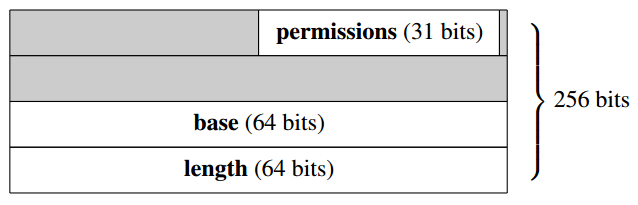
\includegraphics[width=0.8\textwidth]{chericap}
    \caption{CHERI capability \cite{Woodruff:2014:CCM:2665671.2665740}}
    \label{fig:chericap}
  \end{figure}
}
}

\frame{
\frametitle{Capability permissions}
\begin{itemize}
\item Read
\item Write
\item Execute
\item<2-> Enter
%Inspired by the M-Machine
  \begin{itemize}
  \item<3-> When jumped to, it becomes a read and execute capability
  \item<3-> Cannot be used in any other way
  \item<4-> Used by distrusting pieces of code to cross security domains
  \item<5-> Modularisation
  \end{itemize}
\end{itemize}
}

\frame{
\frametitle{Capability machine instructions}
\begin{itemize}
\item<1-> Same instructions as in a normal low-level machine
  \begin{itemize}
  \item<2-> \texttt{\emph<3>{jmp}}, \texttt{\emph<3>{jnz}}, \texttt{move}, \texttt{plus}, \texttt{\emph<3>{load}}, \texttt{\emph<3>{store}}
  \item<3-> Instructions may require capability with certain permission.
    %jmp has to be to an execute capability
    %load has to be through a read capability
    %store has to be through a write capability
  \end{itemize}
\item<4-> Capability manipulation instructions
  \begin{itemize}
  \item<5-> \texttt{lea}, \texttt{restrict}, \texttt{subseg} 
  \item<6-> No instruction generates new capability
  \item<7-> Manipulation of capabilities cannot result in authority amplification
  \end{itemize}
\end{itemize}
}

\frame{
\frametitle{Capability machine overview}
\begin{itemize}[<+->]
\item Capabilities 
  \begin{itemize}
  \item Permissions
  \item Range of authority
  \end{itemize}
\item Capability aware instructions
\item Heap and registers
  \begin{itemize}
  \item Can contain data and capabilities
    %Capabilities can be distinguished from data using tagging (file or bit in cap).
  \end{itemize}
\end{itemize}
}

\section{Formalisation}
\frame{
\frametitle{Formalisation}
\begin{itemize}[<+->]
\item A mathematical model of the system
\item Allows us to reason formally
\item May make some abstractions
\item Needs to stay true to a real system
\item This formalisation is of a capability machine (not CHERI or the M-Machine)
\end{itemize}
}

\frame{
  \frametitle{Formalisation - Permissions}
  \textbf{Permissions}
  \begin{itemize}
  \item To simplify matters, we only allow certain combinations of permissions
  \item<2-> No permissions, \uncover<3->{read only,} \uncover<4->{read-write,} \uncover<5->{read-execute,} \uncover<6->{enter,} \uncover<7->{read-write-execute}
  \end{itemize}

  \[
    \Perms \defeq \{ \uncover<2->{\noperm,} \uncover<3->{\readonly,} \uncover<4->{\readwrite,} \uncover<5->{\exec,} \uncover<6->{\entry,} \uncover<7->{\rwx}\}
  \]
}

\frame{
  \frametitle{Formalisation - Capabilities}

  \textbf{Capability}
  \begin{itemize}
  \item<2-> Permission
  \item<4-> Range of authority
  \item<7-> Pointer
  \end{itemize}

  \[
    \uncover<5->{\Addrs \defeq \nats}
  \]

  \[
    \Caps \defeq \uncover<3->{\Perms} \uncover<6->{\times \Addrs \times \Addrs} \uncover<8->{\times \Addrs}
  \]
  \uncover<9->{
    Example: $(\entry, 30, 42, 30)$
  }
}

\frame{
  \frametitle{Formalisation - Words and register file}
  \textbf{Words}
  \begin{itemize}
  \item<2-> Capability
  \item<4-> Data (and instructions)
  \item<6-> In the real machine capabilities are tagged 
  \end{itemize}
  \[
    \Words \defeq \uncover<3->{\Caps} \uncover<5->{+ \ints}
  \]
  \uncover<7->{
    \textbf{Register file}
    \begin{itemize}
    \item<8-> Assume finite set of registers $\RegName \ni \pcreg$ 
    \end{itemize}
    \[
      \Regs \defeq \uncover<9->{\RegName \rightarrow \Words}
    \]
  }
}

\frame{
  \frametitle{Formalisation - Heap and configurations}
  \textbf{Heap}
  \begin{itemize}
  \item<2-> Map from $\Addrs$ to $\Words$
    % Example of abstraction
    % Notice there are infinitely many addresses, so the heap is infinite!
    % We only allow finite use of it.
    % This is to avoid dealing with "out of memory" 
  \end{itemize}
  \[
    \Heaps \defeq \uncover<2->{ \Addrs \rightarrow \Words }
  \]

\uncover<3->{
  \textbf{Configuration}
  \begin{itemize}
  \item<4-> Executable configuration
  \item<6-> Successfully halted configuration
  \item<8-> Failed configuration
  \end{itemize}
  \[
    \Confs \defeq\uncover<5->{\Regs \times \Heaps} 
                 \uncover<8->{ + \{ \failed \} }
                 \uncover<7->{ + \{\halted\} \times \Heaps}
  \]
}
}

\begin{frame}
  \frametitle{Formalisation - Instructions}
  \textbf{Syntax}
  \begin{itemize}
  \item<3-> The normal instructions
  \item<5-> The capability manipulation instructions
  \item<7-> Instructions for stopping the machine
  \end{itemize}
  $$\begin{array}{rcl}
   \uncover<2->{\rv     &::=& n \mid \lv }\\
   \Instrs &::=& 
\uncover<4->{
                 \jmp{\lv} \mid \jnz{\lv}{\rv} \mid \move{\lv}{\rv} \mid \\
           &   & \load{\lv}{\hv} \mid \store{\hv}{\lv} \mid \plus{\lv}{\rv}{\rv}
} 
\uncover<6->{
                 \mid\\
           &   & \lea{\lv}{\rv} \mid \restrict{\lv}{\lv}{\rv} \mid  \\
           &   & \subseg{\lv}{\rv}{\rv}
} 
\uncover<8->{
\mid \fail \mid \halt}

  \end{array}$$

\end{frame}

\begin{frame}
  \frametitle{Formalisation - Operational Semantics (1)}
  \textbf{Execution relation}
  \[
    \step \subseteq (\Regs \times \Heaps) \times \Confs
  \]

  \begin{mathpar}
\uncover<2->{
    \inferrule{ \uncover<3->{\memreg(\pcreg) = \stdcap} \\ 
                \uncover<4->{\start \leq \addr \leq \addrend} \\
                \uncover<5->{\perm \in \{ \exec,\rwx\} } }
              { \var{executionAllowed}(\Phi) }
}
    \and
\uncover<6->{
   \inferrule{ \neg \var{executionAllowed}(\Phi) }
             { \Phi \step \uncover<7->{ \failed } }
}
    \and
\uncover<8->{
    \inferrule{ \var{executionAllowed}(\Phi) \\
                \uncover<9->{i = \memheap(a)}}
              { \Phi \step \uncover<10->{\llbracket} \uncover<9->{i} \uncover<10->{\rrbracket(\Phi)} }
} 
  \end{mathpar}
\end{frame}

\begin{frame}
  \frametitle{Formalisation - Operational Semantics (2)}
    \begin{mathpar}
      \inferrule{
        \only<2->{\var{w} = \memheap(\only<2>{r_2}\only<3->{\addr})}
        \only<1>{\phantom{\var{w} = \memheap(r_2)}} \\
%
        \only<3->{\memreg(r_2) = \stdcap}
        \only<1-2>{\phantom{\memreg(r_2) = \stdcap}}\\
%
        \only<4->{\perm \in \{\readonly, \readwrite, \exec, \rwx \}} 
        \only<1-3>{\phantom{\perm \in \{\readonly, \readwrite, \exec, \rwx \} }} \\
%
        \only<5->{\start \leq \addr \leq \addrend} 
        \only<1-4>{\phantom{\start \leq \addr \leq \addrend}}
}
      {\sem{\load{\refreg{r_1}}{\refheap{r_2}}}(\Phi) = 
        \only<6->{\var{updatePc}(}
        \only<1-5>{\phantom{\var{updatePc}(}}
          \only<2->{\updateReg{r_1}{\var{w}}}
          \only<1>{\phantom{\updateReg{r_1}{\var{w}}}}
        \only<6->{)}
        \only<1-5>{\phantom{)}} 
}
    \and
\uncover<11->{
      \inferrule{
        \only<12->{\memreg(r_2) = \stdcap}
        \only<1-11>{\phantom{\memreg(r_2) = \stdcap}} \\
        \only<13->{\var{newPerm} = \decodePerm(\Phi,r_3)}
        \only<1-12>{\phantom{\var{newPerm} = \decodePerm(\Phi,r_3)}}\\
        \only<14->{\var{newPerm} \sqsubseteq \perm}\\
        \only<1-13>{\phantom{\var{newPerm} \sqsubseteq \perm}}\\
        \only<15->{c = (\var{newPerm},\start,\addrend,\addr) }
        \only<1-14>{\phantom{c = (\var{newPerm},\start,\addrend,\addr) }}
      }
      { 
        \sem{\restrict{\refreg{r_1}}{r_2}{r_3}} =
        \only<16->{ \var{updatePc}( }
        \only<1-15>{\phantom{\var{updatePc}( } }
          \updateReg{r_1}{\var{c}}
        \only<16->{  )}
        \only<1-15>{\phantom{  )}}
      }
}
\and
\uncover<7->{
      \inferrule{ 
        \only<8->{\memreg(\pcreg) = \stdcap}
        \only<1-7>{\phantom{\memreg(\pcreg) = \stdcap}} \\
        \only<9->{\var{newPc} = (\perm,\start,\addrend,\addr + 1)}
        \only<1-8>{\phantom{\var{newPc} = (\perm,\start,\addrend,\addr + 1)}}
      }
      { \stdUpdatePc{\Phi} = \updateReg{\pcreg}{\only<10->{\var{newPc}} \only<1-9>{\phantom{\var{newPc}}}} 
      }
}
    \end{mathpar}
\end{frame}

\begin{frame}{Formalisation - Operational Semantics (3)}
  \begin{itemize}[<+->]
  \item Need a $\failed$ case for each of the rules
  \item The operational semantics of the remaining instructions defined in a similar fashion
  \end{itemize}
\end{frame}

\begin{lrbox}{\locstatebox}
\begin{lstlisting}
let f = fun adv =>
          let l = 1 in
          adv();
          assert (l == 1)
\end{lstlisting}
\end{lrbox}

\begin{lrbox}{\tdbox}
  \begin{lstlisting}
fun adv =>
  let c = 0 in
  let td = (fun _ =>
              c := !c + 1) in
  adv(td);
  assert(c >= 0)
\end{lstlisting}

\end{lrbox}

\section{Example program}
\begin{frame}{Example program}

  \begin{itemize}[<+->]
  \item High-level programs - ML style
  \item \texttt{let l = 1 in ...} - allocates a new cell on the heap and sets the value to 1 (assume some trusted malloc exists).
  \item \texttt{assert(l == 1)} - if the assertion is true, then execution continues. If the assertion is false, then an assertion flag (a designated heap cell) is set to 1 and execution halts.
  \end{itemize}

\uncover<4->{
\usebox{\locstatebox}    
\begin{block}<5->{Lemma}
  Given any program \texttt{adv}, \texttt{f(adv)} either runs forever, ends up in the \failed{} configuration, or halts in a configuration where the assertion flag is 0.
\end{block}
}
\end{frame}

\begin{comment}
\begin{frame}{Example: local state}
\usebox{\tdbox}
\end{frame}
\end{comment}

\section{Logical Relation}
\frame{
\frametitle{Logical Relation - What is it }
\textbf{Logical relations in general}
\begin{itemize}[<+->]
\item Strong proof method
\item Used to show properties about programs
\item Designed such that any program in the relation has a certain property
\item Can be used when a direct proof does not suffice
  \begin{itemize}
  \item e.g., strong normalisation for STLC
  \end{itemize}
\item Can be used to reason about programs written in ``real'' programming languages
\item Extensional - not interested in what happens doing the execution, only interested in the result
\end{itemize}
}

\frame{
  \frametitle{Logical Relation}
  \textbf{What we hope to achieve}
  \begin{itemize}[<+->]
  \item Any program will respect the limitations of the capability system.
  \end{itemize}
}

\frame{
  \frametitle{Logical Relation}
  \textbf{The property of this logical relation}\\
  \begin{itemize}
  \item<2-> Any capability such that
    \begin{itemize}
    \item<3-> when executed in a ``well-behaved'' register-file, and
    \item<3-> a heap that satisfies \alert<8->{certain invariants}\uncover<4->{, then}
    \item<4-> the execution will either
      \begin{itemize}
      \item<5-> diverge\uncover<6->{,}
      \item<6-> end up in the \failed{} configuration\uncover<7->{, or}
      \item<7-> halt where the heap still satisfies the invariants
      \end{itemize}
    \end{itemize}
\end{itemize}

%Strong proof technique/method
%Used to prove properties about programs
%Can be used instead of direct proof
%Semantic way of reasnong
%(as opposed to syntactic)
%Designed such that any program in the relation has a certain property
%Could be type safety for STLC
%Here any "program" in the relation can be put into "good" context and run which will produce a result that retains all heap invariants.
%Intentional - only interested in the end result. (as opposed to extensional?) (ask Dominique about the terms here)
}


\begin{frame}{Logical Relation - Worlds, modelling the heap}

\begin{overlayarea}{\textwidth}{3cm}
\only<1-2>{\textbf{World}}
\only<1-2>{
\begin{itemize}
\item<1-2> Collection of regions with invariants (e.g.\ $h(27) \mapsto 5 $)
\item<2> Model of the heap
\end{itemize}
}
\only<3-7>{\textbf{Heap satisfaction}}
\only<3-7>{
  \begin{itemize}
  \item<3-> Regions model parts of the heap
  \item<4-> Non-overlapping
  \item<7> $h : W$ 
  \end{itemize}
}
\only<8->{\textbf{Future World}}
\only<8-9>{
  \begin{itemize}
  \item<8-9> Heap changes over time, worlds have to cope with this:
  \item $\onslide<9->{W' \future} W$
    \begin{itemize}
    \item<8-9> Same regions as before
    \item<9> New region(s)
    \end{itemize}
  \end{itemize}
}
\only<10->{
  \begin{itemize}
  \item<10-> Old regions model the same parts of the heap as before
  \item<11-> New part model new part of the heap
  \end{itemize}
}

\end{overlayarea}
\begin{overprint}
  \onslide<1>
  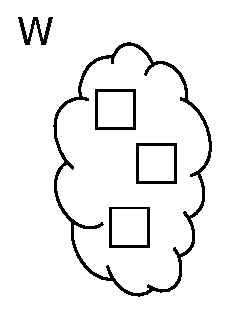
\includegraphics{world1.eps}
  \onslide<2>
  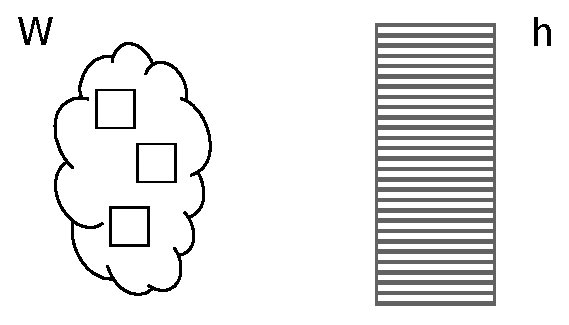
\includegraphics{world2.eps}
  \onslide<3>
  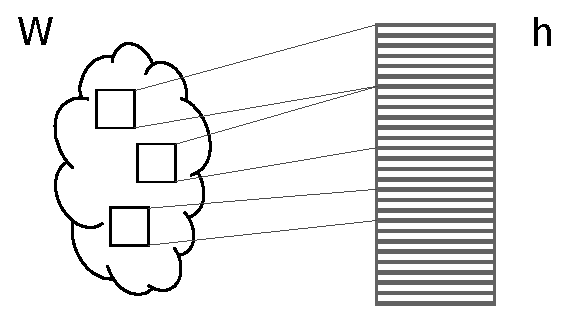
\includegraphics{world3.eps}
  \onslide<4>
  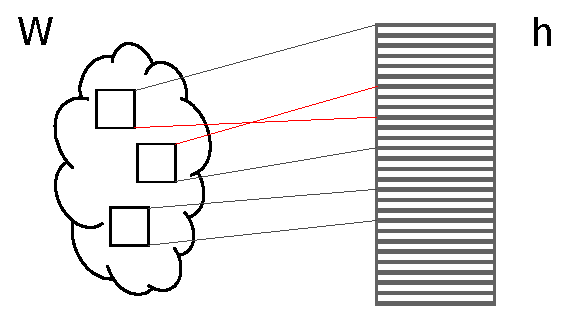
\includegraphics{world4.eps}
  \onslide<5>
  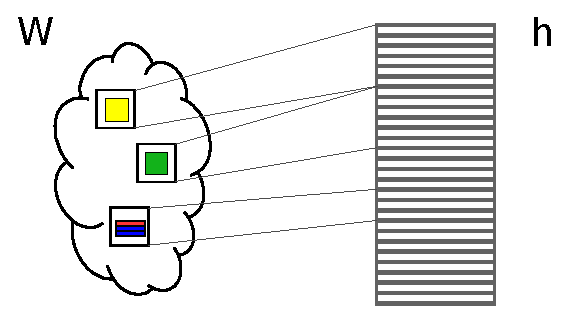
\includegraphics{world5.eps}
  \onslide<6>
  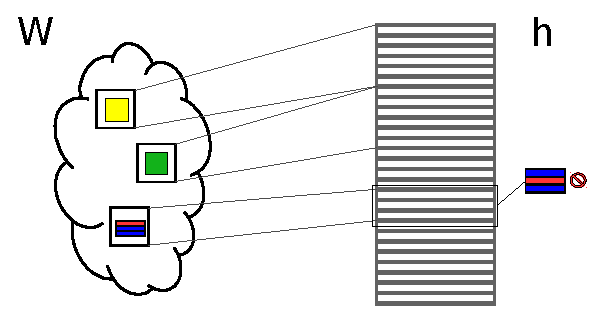
\includegraphics{world6.eps}
  \onslide<7>
  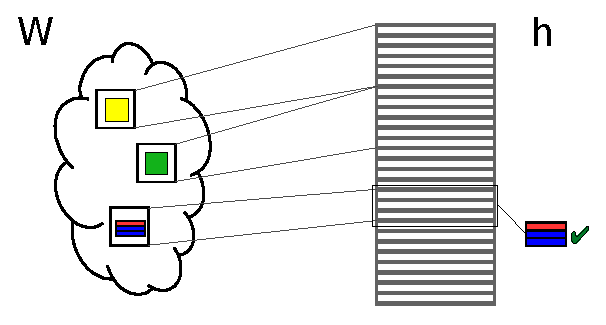
\includegraphics{world12.eps}
  \onslide<8>
  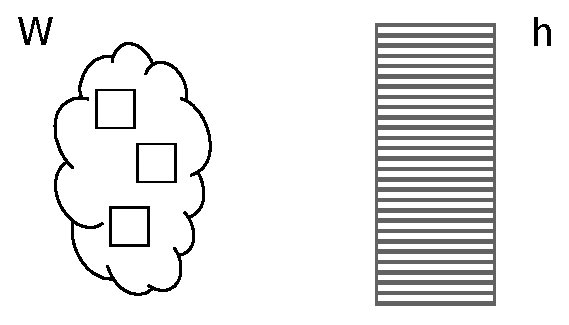
\includegraphics{world2.eps}
  \onslide<9>
  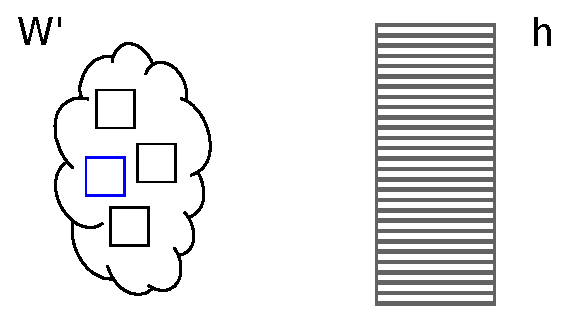
\includegraphics{world11.eps}
  \onslide<10>
  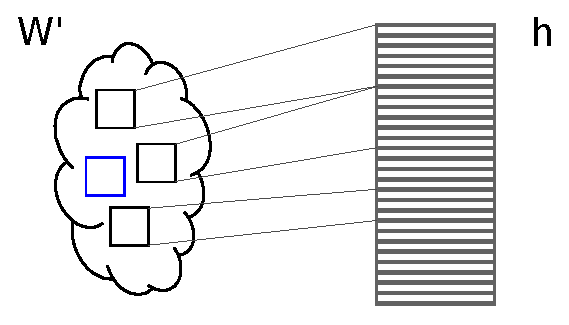
\includegraphics{world9.eps}
  \onslide<11>
  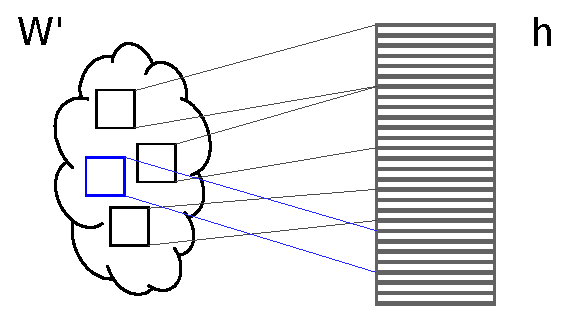
\includegraphics{world10.eps}
\end{overprint}

\end{frame}
\begin{comment}
  \[
\Rel \defeq \{ R \subseteq \States \times \States \mid R \text{ is reflexive and transitive}  \}
\]
\[
\Regions \defeq (\States \times \Rel \times (\States \fun (\Worlds \monnefun 2^\HeapSegments)))
\]
\[
\Worlds \defeq \RegionNames \finparfun \Regions
\]

\end{comment}
\frame{
  \frametitle{Logical Relation}
  \textbf{The property of this logical relation}\\
  \begin{itemize}
  \item Any capability such that
    \begin{itemize}
    \item when executed in a ``well-behaved'' register-file, and
    \item a heap that satisfies certain invariants, then
    \item \alert<2>{the execution will either}
      \begin{itemize}
      \item \alert<2>{diverge,}
      \item \alert<2>{end up in the \failed{} configuration, or}
      \item \alert<2>{halt where the heap still satisfies the invariants}
      \end{itemize}
    \end{itemize}
\end{itemize}
}
\frame{
\frametitle{ Logical Relation - Observation relation }
\textbf{Property}
\begin{itemize}
\item the execution will either
  \begin{itemize}
  \item \textbf<3>{diverge},
  \item \textbf<4>{end up in the \failed{} configuration}, or
  \item \textbf<2>{halt where the heap still satisfies the invariants}
  \end{itemize}
\end{itemize}

\begin{align*}
  \observations \defeq \lambda W \ldotp \{ (\reg,h) \mid
  \begin{aligned}[t]
    & \only<1>{ \phantom{(\forall h' \ldotp (\reg,h) \step^* (\halted,h')} }  
     \only<2->{(\forall h' \ldotp (\reg,h) \step^* (\halted,h')}  \\
    & \only<1>{ \phantom{\qquad \Rightarrow \exists W' \future W \ldotp  \heapSat[h']{}{W'}) \lor} } 
     \only<2->{\qquad \Rightarrow \exists W' \future W \ldotp  \heapSat[h']{}{W'})} \only<2-5>{\lor} \only<6>{\}}\\
    & \only<3-5>{(\reg,h) \Downarrow \lor}
      \only<1-2>{\phantom{(\reg,h) \Downarrow \lor} }    \\
    & \only<4-5>{(\reg,h)\step^*\failed\} }
      \only<1-3>{\phantom{(\reg,h)\step^*\failed\}} } 
  \end{aligned}
\end{align*}
}

\frame{
  \frametitle{Logical Relation}
  \textbf{The property of this logical relation}\\
  \begin{itemize}
  \item \alert<2>{Any capability such that}
    \begin{itemize}
    \item \alert<2>{when executed in a ``well-behaved'' register-file, and}
    \item \alert<2>{a heap that satisfies certain invariants, then}
    \item \alert<2>{the execution will either}
      \begin{itemize}
      \item diverge,
      \item end up in the \failed{} configuration, or
      \item halt where the heap still satisfies the invariants
      \end{itemize}
    \end{itemize}
\end{itemize}
}

\frame{
\frametitle{Logical Relation - Expression relation}
\begin{itemize}
  \item Any capability such that
    \begin{itemize}
    \item \textbf<2>{when executed in a ``well-behaved'' register-file}, and
    \item \textbf<3>{a heap that satisfies certain invariants}, then
    \item \textbf<4>{the execution will either ...}
    \end{itemize}
\end{itemize}
\begin{align*}
  \stder \defeq & \lambda W \ldotp \{ \var{c} \mid 
  \begin{aligned}[t]
    & \only<1>{\phantom{\forall \reg \in \stdrr(W) \ldotp} }
      \only<2->{\forall \reg \in \stdrr(W) \ldotp} \\
    & \only<1-2>{\phantom{ \quad \forall \heapSat[h]{ }{W} \ldotp} }
      \only<3->{\quad \forall \heapSat[h]{ }{W} \ldotp} \\
    & \only<4->{\qquad (\reg\update{\pcreg}{\var{c}},h) \in \observations(W) \} }
      \only<1-3>{\phantom{\qquad (\reg\update{\pcreg}{\var{c}},h) \in \observations(W) \} } }
  \end{aligned}
\end{align*}
}

\frame{
\frametitle{Logical Relation - Register-file relation}
\textbf{``Well-behaved'' register-file}
\begin{itemize}
\item<2-> All registers but the $\pcreg$-register
  \begin{itemize}
  \item<3-> $\pcreg$ was overwritten in the $\stder$ anyway
  \end{itemize}
\item<4-> should contain a ``well-behaved'' word
\end{itemize}
\begin{align*}
  \stdrr \defeq & \lambda W \ldotp \{ \reg \mid 
                  \begin{aligned}[t]
                    & \only<1>{\phantom{\forall r \in \RegName \setminus \{\pcreg\} \ldotp} }
                      \only<2->{\forall r \in \RegName \setminus \{\pcreg\} \ldotp} \\
                    & \only<1-3>{\phantom{ \quad  \reg(r) \in \stdvr(W) \} }}
                      \only<4->{\quad  \reg(r) \in \stdvr(W) \}}
                  \end{aligned}
\end{align*}
}

\frame{
\frametitle{Logical Relation - Value relation}
\textbf{``Well-behaved words''}
\begin{align*}
  \stdvr &\defeq \lambda \; W \ldotp 
           \begin{aligned}[t]
             & \{ i \mid i \in \ints \} 
             \union \\
             & \{ \stdcap[\noperm] \} 
             \union \\
             & \{ \stdcap[\readonly] \mid 
                \only<1>{\phantom{\readCond{}(\start,\addrend,W)} }
                \only<2->{\readCond{}(\start,\addrend,W)}
                  \} \union \\
             & \{ \stdcap[\readwrite] \mid 
             \begin{aligned}[t]
               &\only<1>{\phantom{\readCond{}(\start,\addrend,W)} }
                \only<2->{\readCond{}(\start,\addrend,W)}
                \land \\
               &\only<1-2>{\phantom{\writeCond{}(\start,\addrend,W)} }
                \only<3->{\writeCond{}(\start,\addrend,W)}
                \} \union
             \end{aligned}
\\
             & \{ \stdcap[\exec] \mid 
             \begin{aligned}[t]
               &\only<1>{\phantom{\readCond{}(\start,\addrend,W)} }
                \only<2->{\readCond{}(\start,\addrend,W)} \land \\
               &\only<1-3>{\phantom{\execCond{}(\start,\addrend,W)} }
                \only<4->{\execCond{}(\start,\addrend,W)} \} \union
             \end{aligned}
              \\
             % For the entry case a capability is acceptable, if we can change it to an execute permission and put it as the pc and we otherwise have valid words in the registers, then the register file should be valid.
             & \{ \stdcap[\entry] \mid 
                \only<1-4>{\phantom{\entryCond{}(\start,\addrend,\addr,W)} }
                \only<5->{\entryCond{}(\start,\addrend,\addr,W)} \union \\
             & \{ \stdcap[\rwx] \mid 
             \begin{aligned}[t]
               & \only<1>{\phantom{\readCond{}(\start,\addrend,W)} }
                 \only<2->{\readCond{}(\start,\addrend,W)}\land \\
               & \only<1-2>{\phantom{\writeCond{}(\start,\addrend,W)} }
                 \only<3->{\writeCond{}(\start,\addrend,W)} \land \\
               & \only<1-3>{\phantom{\execCond{}(\start,\addrend,W)} }
                 \only<4->{\execCond{}(\start,\addrend,W)} \}
             \end{aligned}
           \end{aligned}
\end{align*}
}


\begin{frame}{Logical Relation - Execute and enter conditions}
  \begin{overlayarea}{\textwidth}{2.3cm}
    \only<1-4>{
      \textbf{Execution condition}
      \begin{itemize}
      \item<2-4> May be used at any point in the future
      \item<3-4> Can be executed from any address in the range of authority
      \item<4>   Should produce a ``well-behaved'' result, i.e., it should be in the $\stder$-relation
      \end{itemize}
    }
    \only<5->{
      \textbf{Enter condition}
      \begin{itemize}
      \item<6-> May be used at any point in the future
      \item<7-> Can only be executed from the specified address
      \item<8-> Should produce a ``well-behaved'' result, i.e., it should be in the $\stder$-relation
      \end{itemize}
    }
  \end{overlayarea}
  \begin{overprint}
\onslide<1-4>
    \begin{align*}
      & \execCond{}(\start,\addrend,W) \defeq \\
      & \only<1>{\phantom{\qquad  \forall W' \future W \ldotp} }
        \only<2-4>{\qquad  \forall W' \future W \ldotp} \\
      & \only<1-2>{\phantom{\qquad \quad \forall \addr \in [\start,\addrend] \ldotp} }
        \only<3-4>{\qquad \quad \forall \addr \in [\start,\addrend] \ldotp} \\
      & \only<1-3>{\phantom{\qquad \qquad (\exec,\start,\addrend,\addr) \in \stder(W')} }
        \only<4>{\qquad \qquad (\exec,\start,\addrend,\addr) \in \stder(W')}
    \end{align*}
\onslide<5->
    \begin{align*}
      & \entryCond{}(\start,\addrend,\addr,W) \defeq \\
      & \only<5>{\phantom{\qquad  \forall W' \future W \ldotp} }
        \only<6->{\qquad  \forall W' \future W \ldotp} \\
      & \only<5-7>{\phantom{\qquad \qquad (\exec,\start,\addrend,\addr) \in \stder(W')} }
        \only<8->{\qquad \qquad (\exec,\start,\addrend,\addr) \in \stder(W')}
    \end{align*}
  \end{overprint}

\end{frame}

\frame{
\frametitle{Logical Relation - Read and write conditions}
\begin{overlayarea}{\textwidth}{2cm}
\only<1-3>{
\textbf{Read condition}
\begin{itemize}
\item<1-> World models heap, so it describes what we might read
\item<2-> Some region should govern the part of the heap we can read from
\item<3-> The region may govern a larger part of the heap
\end{itemize}
}
\only<4-8>{
\textbf{Read condition}
\begin{itemize}
\item<4-> The region should be subset of the standard region $\iota_{\start',\addrend'}$
\item<8-> Intuition:
  \begin{itemize}
  \item<8-> If untrusted code got this capability, then it should only be able to read ``well-behaved'' words.
  \end{itemize}
\end{itemize}
}

\only<9-10>{
\textbf{Write condition}
\begin{itemize}
\item<9-> World should describe what we are allowed write
\item<10-> Some region governs the part of the heap we may write to

\end{itemize}
}
\only<11->{
\textbf{Write condition}
\begin{itemize}
\item<11-> The region should be \emph{superset} of the standard region $\iota_{\start',\addrend'}$
\item<12-> Intuition:
  \begin{itemize}
  \item<12-> If untrusted code got this capability, then it can at least write something well-behaved, but also other things.
  \end{itemize}
\end{itemize}
}
\end{overlayarea}

\begin{overlayarea}{\textwidth}{3cm}
\only<1-8>{
\begin{align*}
  &\readCond{}(\start,\addrend, W) \defeq \\
  & \only<1>{\phantom{\qquad\quad \exists r \in \RegionNames \ldotp} }
    \only<2-9>{\qquad\quad \exists r \in \RegionNames \ldotp} \\
  & \only<1-2>{\phantom{\qquad\qquad \exists [\start',\addrend'] \supseteq [\start,\addrend] \ldotp} } 
    \only<3-9>{\qquad\qquad \exists [\start',\addrend'] \supseteq [\start,\addrend] \ldotp} \\
  & \only<1-3>{\phantom{\qquad\qquad \quad W(r) \subseteq \iota_{\start',\addrend'}} }
    \only<4-9>{\qquad\qquad \quad W(r) \subseteq \iota_{\start',\addrend'}}
\end{align*}
}
\only<9->{
\begin{align*}
  & \writeCond{}(\start,\addrend, W) \defeq \\
  & \only<9>{\phantom{\qquad\quad \exists r \in \RegionNames \ldotp} }
    \only<10->{\qquad\quad \exists r \in \RegionNames \ldotp} \\
  & \only<9>{\phantom{\qquad\qquad \exists [\start',\addrend'] \supseteq [\start,\addrend] \ldotp} } 
    \only<10->{\qquad\qquad \exists [\start',\addrend'] \supseteq [\start,\addrend] \ldotp} \\
  & \only<9-10>{\phantom{\qquad\qquad \quad W(r) \supseteq \iota_{\start',\addrend'}} }
    \only<11->{\qquad\qquad \quad W(r) \supseteq \iota_{\start',\addrend'}}
\end{align*}
}
\end{overlayarea}
\begin{itemize}
\item<5-> $\iota_{\start',\addrend'}$ is a standard region that requires
  \begin{itemize}
  \item<6-> Range of heap segment to be $[\start',\addrend']$
  \item<7-> All the words in the heap segment should be in the $\stdvr$-relation
  \end{itemize}
\end{itemize}
}


\frame{
\frametitle{Fundamental theorem of logical relations}
\begin{overprint}
\onslide<1-3>
\begin{lemma}[FTLR] 
  For all $W \in \Worlds$ and $c \in Caps$,
  \[
    c \in \stder(W).
  \]
\end{lemma}
\onslide<2-3>{
  \begin{itemize}
  \item<2-> The $\pcreg$-register can be accessed like any other register
  \item<3> Capability must behave when used for read/write
  \end{itemize}
}
\onslide<4>
\begin{lemma}[FTLR] 
  For all $W \in \Worlds$, $\perm \in \Perms$, and $\start,\addrend,\addr \in \Addrs$, \\

  if
  \[ 
    \perm = \exec\text{ and }\readCond{W,\start,\addrend},
  \]
  or
  \[
    \perm = \rwx \text{ and } \var{read\text{-/}writeCond}(W,\start,\addrend)
  \]
  then 
  \[
    (\perm, \start, \addrend, \addr) \in \stder(W).
  \]
\end{lemma}
\end{overprint}

}

\section{Example revisited}

\begin{frame}{Example: local state revisited}
\begin{overprint}
\onslide<1>
\begin{block}{Lemma}
  Given any program \texttt{adv}, \texttt{f(adv)} either runs forever, ends up in the \failed{} configuration, or halts in a configuration where the assertion flag is 0.
\end{block}

\onslide<2-9>
Proof sketch
\begin{itemize}
\item<2-> Assuming \texttt{adv} is only code and given as enter capability
\item<3-> Run program until just after the jump to \texttt{adv}
\item<4-> Define world with the following regions:
  \begin{itemize}
  \item<5-> \texttt{f} code remains unchanged
  \item<6-> \texttt{l} remains 1
  \item<7-> standard region governs \texttt{adv}
  \item<8-> assertion flag is 0
  \end{itemize}
\item<9-> Use FTLR on \texttt{adv} capability 
\end{itemize}

\onslide<10-15>
Proof sketch (continued)
\begin{itemize}
\item<10-> Use FTLR on \texttt{adv} capability
\item<11-> By design, the heap satisfies the world
\item<12-> Register-file in $\stdrr$-relation:
  \begin{itemize}
  \item<13-> All registers but two contain 0, so trivial.
  \item<14-> One is $\pcreg$-register, so we don't care about it.
  \item<15-> The other is the continuation (passed as enter capability), so $\entryCond{}$ must hold
  \end{itemize}
\end{itemize}

\onslide<16-19>
Proof sketch (continued)
\begin{itemize}
\item<16-> World highlights:
  \begin{itemize}
  \item \texttt{f} code remains unchanged
  \item \texttt{l} remains 1
  \item assertion flag is 0
  \end{itemize}
\item<16-> The continuation satisfies $\entryCond{}$:
  \begin{itemize}
  \item<17-> In a future world, the continuation must be in $\stder$
  \item<18-> Executing from continuation, \texttt{l} is still 1, so assertion does not fail.
  \item<19-> Execution halts and assertion flag is 0
  \end{itemize}

\end{itemize}
\onslide<20-21>
Proof sketch (continued)
\begin{itemize}
\item<20-> Backtracking a lot, we have just shown that the register-file was in the $\stdrr$-relation
\item<21-> By $\mathtt{adv} \in \stder$: execution diverges, fails, or terminates without the assertion failing.
\end{itemize}

\onslide<22>
\begin{block}{Lemma}
  Given any program \texttt{adv}, \texttt{f(adv)} either runs forever, ends up in the \failed{} configuration, or halts in a configuration where the assertion flag is 0.
\end{block}
\begin{overlayarea}{\textwidth}{0.5cm}
  
\end{overlayarea}

\end{overprint}
\begin{overlayarea}{\textwidth}{3cm}
  \usebox{\locstatebox}
\end{overlayarea}
\end{frame}


\begin{lrbox}{\continuationbox}
  \begin{lstlisting}
let f = fun adv =>
  let l = 0 in
  adv();
  assert(l == 0);
  l := 1;
  adv()
  \end{lstlisting}
\end{lrbox}

\section{Current work}

\frame{
\frametitle{What are we working on now?}
\usebox{\continuationbox}
\pause
\begin{itemize}
\item Assuming standard calling convention, can we show that the assertion never fails?
\pause
  \begin{itemize}
  \item No,\pause{} \texttt{adv} may save the continuation from the first
    call
  \end{itemize}
\end{itemize}
\pause
\textbf{Local capabilities}\pause
\begin{itemize}
\item \emph{local}/\emph{global} capabilities\pause
\item \emph{permit write local} capabilities\pause
\item \emph{Local} capabilities can only be stored through \emph{permit write local} capabilities
\end{itemize}
}

\frame{
  \frametitle{Questions?}

}

\frame{
\frametitle{References}
  \bibliographystyle{plainnat}
  \bibliography{refs}
}

\end{document}